\part{Graph and Network Theory}
	\chapter{Basic concepts}
		\section{Graph}
			\begin{definition}[Graph]
				A \textbf{graph} G consists of a finite set $V(G)$ on vertices, a finite set $E(G)$ on edges and an \textbf{incident relation} than associates with any edge $e\in E(G)$ an unordered pair of vertices not necessarily distinct called \textbf{ends}.
			\end{definition}

			For example, the following graph\\
			\begin{figure}[!ht]
				\centering
				\begin{tikzpicture}[node distance = 1.7cm]
					\node (v_2) [circleNode] {$v_2$};
					\node (v_3) [circleNode, right of = v_2] {$v_3$};
					\node (v_1) [circleNode, below of = v_2] {$v_1$};
					\node (v_4) [circleNode, below of = v_3] {$v_4$};
					\node (v_5) [circleNode, right of = v_3] {$v_5$};
					\node (v_6) [circleNode, below of = v_5] {$v_6$};
					\draw [link] (v_2) -- node [left] {$e_2$} (v_1);
					\draw [link] (v_2) -- node [below] {$e_5$} (v_4);
					\draw [link] (v_1) to [out = 180, in = 270, looseness = 5] node [right] {$e_1$} (v_1);
					\draw [link] (v_2) to [out = 45, in = 135] node [above] {$e_3$} (v_3);
					\draw [link] (v_2) -- node [above] {$e_4$} (v_3);
					\draw [link] (v_3) -- node [right] {$e_6$} (v_1);
					\draw [link] (v_5) -- node [right] {$e_7$} (v_6);
				\end{tikzpicture}			
			\end{figure}\\
			can be represented as\\
			\begin{align}
				V = V(G) = \{v_1, v_2, v_3, v_4, v_5, v_6\} \\
				E = E(G) = \{e_1, e_2, e_3, e_4, e_5, e_6, e_7\}\\
				e_1 = v_1v_2, e_2 = v_2v_4, ...
			\end{align}

			\begin{definition}[loop, parallel, simple graph]
				An edge with identical ends is called a \textbf{loop}, Two edges having the same ends are said to be \textbf{parallel}, A graph without loops or parallel edges is called \textbf{simple graph}
			\end{definition}

			\begin{definition}[adjacent]
				Two edges of a graph are \textbf{adjacent} if they have a common end, two vertices are \textbf{adjacent} if they are jointed by an edge.
			\end{definition}

		\section{Subgraph}
			\begin{definition}[subgraph]
				Given two graphs $G$ and $H$, $H$ is a \textbf{subgraph} of $G$ if $V(H)\subseteq V(G)$, $E(H)\subseteq E(G)$ and an edge has the same ends in $H$ as it does in $G$. Furthermore, if $E(H)\neq E(G)$ then $H$ is a proper subgraph.
			\end{definition}
			
			\begin{definition}[spanning]
				A subgraph $H$ on $G$ is \textbf{spanning} if $V(H) = V(G)$
			\end{definition}

			\begin{definition}[vertex-induced, edge-induced]
				For a subset $V^{'}\subseteq V(G)$ we define an \textbf{vertex-induced} subgraph $G[V^{'}]$ to be the subgraph with vertices $V^{'}$ and those edges of $G$ having both ends in $V^{'}$. The \textbf{edge-induced} subgraph $G[E^{'}]$ has edges $E^{'}$ and those vertices of $G$ that are ends to edges in $E^{'}$.
			\end{definition}

			\notice{If we combine node-induced or edge-induced subgraphs $G(V^{'})$ and $G(V - V^{'})$, we cannot always get the entire graph.}

			\begin{definition}[degree]
				Let $v\in V(G)$, then the \textbf{degree} of $v\in V(G)$ denote by $d_G(v)$ is defines to be the number of edges incident of $v$. Loops counted twice.
			\end{definition}			

			\begin{theorem}
				For any graph $G=(V, E)$
				\begin{equation}
					\sum_{v\in V}d(v) = 2|E|
				\end{equation}			
			\end{theorem}

			\begin{proof}
				$\forall$ edge $e=\mu v$ with $\mu \neq v$, $e$ is  and counted once for $\mu$ and once for $v$, a total of two altogether. If $e=\mu \mu$, a loop, then it is counted twice for $\mu$			
			\end{proof}

			\begin{problem}
				Explain clearly, what is the largest possible number of vertices in a graph with 19 edges and all vertices of degree at least 3. Explain why this is the maximum value.
			\end{problem}

			\begin{solution}
				The maximum number is 12.
			\end{solution}

			\begin{proof}
				First we prove 12 vertices is possible, then we prove 13 vertices is not possible
				\begin{itemize}
					\item The following graph contains 12 vertices and 18 edges, each vertex has a degree of 3.\\
						\begin{figure}[!ht]
							\centering
							\begin{tikzpicture}[node distance=1cm]
								\node (1) [solidNode] {};
								\node (2) [solidNode, below of=1] {};
								\node (3) [solidNode, below of=2] {};
								\node (4) [solidNode, below of=3] {};
								\node (5) [solidNode, below of=4] {};
								\node (6) [solidNode, below of=5] {};
								\node (7) [solidNode, right of=1, xshift=2cm] {};
								\node (8) [solidNode, right of=2, xshift=2cm] {};
								\node (9) [solidNode, right of=3, xshift=2cm] {};
								\node (10) [solidNode, right of=4, xshift=2cm] {};
								\node (11) [solidNode, right of=5, xshift=2cm] {};
								\node (12) [solidNode, right of=6, xshift=2cm] {};
								\draw [link] (1) -- (7);
								\draw [link] (1) -- (8);
								\draw [link] (1) -- (9);
								\draw [link] (2) -- (8);
								\draw [link] (2) -- (9);
								\draw [link] (2) -- (10);
								\draw [link] (3) -- (9);
								\draw [link] (3) -- (10);
								\draw [link] (3) -- (11);
								\draw [link] (4) -- (10);
								\draw [link] (4) -- (11);
								\draw [link] (4) -- (12);
								\draw [link] (5) -- (11);
								\draw [link] (5) -- (12);
								\draw [link] (5) -- (7);
								\draw [link] (6) -- (12);
								\draw [link] (6) -- (7);
								\draw [link] (6) -- (8);
							\end{tikzpicture}
						\end{figure}
					\item For 13 vertices and each vertex has a degree of at least 3 will require at least
						\begin{equation}
							2|E| = \sum_{v \in V}d(v) \ge 3 \times |N| = 3 \times 13 \Rightarrow |E| \ge 19.5 > 19
						\end{equation}
						edges, i.e., 13 vertices is not possible.
				\end{itemize}
			\end{proof}

			\begin{corollary}
				Every graph has an even number of odd degree vertices.
			\end{corollary}

			\begin{proof}
				\begin{equation}
					V = V_E\cup V_O \Rightarrow 
					\sum_{v\in V}d(v) = \sum_{v\in V_E} d(v) + \sum_{v\in V_O}d(v) = 2|E|
				\end {equation}			
			\end{proof}

	\chapter{Paths, Trees, and Cycles}
		\section{Walk}
			\begin{definition}[walk]
				A \textbf{walk} in a graph $G$ is a finite sequence $w=v_0e_1v_1e_2...e_kv_k$, where for each $e_i=v_{i-1}v_i$ the edge and its ends exists in $G$. We say that walk $v_0$ to $v_k$ on $(v_0, v_k)$-walk.
			\end{definition}

			\begin{example}
				\begin{equation}
					w = v_2e_4v_3e_4v_2e_5v_3
				\end{equation}
				is a walk, or $(v_2, v_3)$-walk				
			\end{example}

			\begin{definition}[origin, terminal, internal, length]
				For $(v_0, v_k)$-walk, The vertices $v_0$ and $v_k$ are called the \textbf{origin} and the \textbf{terminal} of the walk w, $v_1..v_{k-1}$ are called \textbf{internal} vertices. The integer $k$ is the \textbf{length} of the walk. Length of $w$ equals to the number of edges.
			\end{definition}
			
			We can create a reverse walk $w^{-1}$ by reversing $w$.
			\begin{equation}
				w^{-1} = v_ke_kv_{k-1}e_{k-1}...e_2v_1
			\end{equation}
			(The reverse walk is guaranteed to exist because it is an undirected graph)

			Given two walks $w$ and $w'$ we can create a third walk denoted by $ww'$ by concating $w$ and $w'$. The new walk's origin is the same as terminal.

		\section{Path and Cycle}
			\begin{definition}[trail]
				A \textbf{trail} is a walk with no repeating edges. e.g., $v_3e_4v_2e_5v_3$
			\end{definition}
			
			\begin{definition}[path]
				A \textbf{path} is a trail with no repeating vertices. e.g., $v_3e_4v_2$
			\end{definition}
			
			\notice{Paths $\subseteq$ Trails $\subseteq$ Walks}

			\begin{definition}[closed, cycle]
				A path is \textbf{closed} if it has positive length and its origin and terminal are the same. e.g., $v_1e_2v_2e_4v_3e_3v_1$. A closed trail where origin and internal vertices are distinct is called a \textbf{cycle} (The only time a vertex is repeated is the origin and terminal)
			\end{definition}
			
			\begin{definition}[even/odd cycle]
				A cycle is \textbf{even} if it has a even number of edges otherwise it is \textbf{odd}.
			\end{definition}

			\begin{problem}
				Prove that if $C_1$ and $C_2$ are cycles of a graph, then there exists cycles $K_1, K_2, ..., K_m$ such that $E(C_1)\Delta E(C_2) = E(K_1)\cup E(K_2) \cup...\cup E(K_m)$ and $E(K_i)\cap E(K_j)=\emptyset, \forall i \neq j$. (For set $X$ and $Y$, $X\Delta Y = (X-Y)\cup(Y-X)$, and is called the symmetric difference of $X$ and $Y$)
			\end{problem}

			\begin{proof}
				Proof by constructing $K_1, K_2, ... K_m$. Denote 
				\begin{align}
					C_1 & = v_{11}e_{11}v_{12}e_{12}v_{13}e_{13}...v_{1n}e_{1n}v_{11}\\
					C_2 & = v_{21}e_{21}v_{22}e_{22}v_{23}e_{23}...v_{2k}e_{2k}v_{21}
				\end{align}
				Assume both cycle start at the same vertice, $v_{11} = v_{12}$. (If there is no intersected vertex for $C_1$ and $C_2$, just simply set $K_1 = C_1$ and $K_2 = C_2$)\\
				The following algorithm can give us all $K_j, j=1, 2, ... , m$ by constructing $E(C_1)\Delta E(C_2)$.  Also, the complexity is $O(mn)$, which makes the proof doable.\\
				\begin{algorithm}[!ht]
					\caption{Find $K_1, K_2, ... K_m$ by constructing $E(C_1)\Delta E(C_2)$}
					\begin{algorithmic}[1]
						\REQUIRE Graph $G$, cycle $C_1$ and $C_2$
						\ENSURE $K_1, K_2, ... K_m$
						\STATE Initial, $K \gets \emptyset$, $j = 1$
						\STATE Set temporary storage units, $v_o \gets v_{11}$, $v_t \gets \emptyset$
						\FOR {$i = 1, 2, ..., n$}
							\IF {$e_{1i} \in C_2$}
								\IF {$v_o \ne v_{1i}$}
									\STATE $v_t \gets v_{1i}$
									\STATE concate $(v_o, v_t)$-path $\subset C_1$ and $(v_o, v_t)$-path $\subset C_2$ to create a new $K_j$
									\STATE Append $K$ with $K_j$, $K \gets K \cup K_j$
									\STATE Reset temporary storage unit. $v_o \gets v_{1(i+1)}$ (or $v_{11}$ if $i = n$), $v_t \gets \emptyset$
								\ELSE
									\STATE $v_o \gets v_{1(i+1)}$ (or $v_{11}$ if $i = n$)
								\ENDIF
							\ENDIF
						\ENDFOR
					\end{algorithmic}
				\end{algorithm}\\
				Now we prove that $K_i\cap K_j = \emptyset, \forall i \ne j$. For each $K_j$, it is defined by two $(v_o, v_t)$-paths in the algorithm. From the algorithm we know that all the edges in $(v_o, v_t)$-path in $C_1$ are not intersecting with $C_2$, because if the edge in $C_1$ is intersected with $C_2$, either we closed the cycle $K_j$ before the edge, or we updated $v_o$ after the edge (start a new $K_j$ after that edge). By definition of cycle, all the $(v_o, v_t)$-path that are subset of $C_1$ are not intersecting with each other, as well as all the $(v_o, v_t)$-path that are subset of $C_2$. Therefore, $K_i\cap K_j = \emptyset, \forall i \ne j$.
			\end{proof}
			
			\begin{definition}[connected vertices]
				Two vertices $u$ and $v$ in a graph are said to be \textbf{connected} if there is a path between $u$ and $v$.
			\end{definition}
			
			\begin{definition}[component]
				Connectivity between vertices is an equivalence relation on $V(G)$, if $V_1, ... V_k$ are the corresponding equivalent classes then $G[V_1]...G[V_k]$ are \textbf{components} of G. If graph has only one component, then we say the graph is connected. A graph is connected iff every pair of vertices in G are connected, i.e., there exists a path between every pair of vertices.
			\end{definition}

			\begin{problem}
				If $G$ is a simple graph with at least two vertices, prove that $G$ has two vertices with the same degree.
			\end{problem}

			\begin{proof}
				A simple graph can only be connected or not connected.
				\begin{itemize}
					\item If $G$ is connected, i.e., for all vertices, the degree is greater than 0. Also the graph is simple, for a graph with $|N|$ vertices, the degree of each vertex is less or equal to $|N| - 1$ (cannot have loop or parallel edge). For $|N|$ vertices, to make sure there is no two vertices that has same degree, it will need $|N|$ options for degrees, however, we only have $|N| - 1$ option. According to pigeon in holes principle, there has to be at least two vertices with the same degree.
					\item If $G$ is not connected, i.e., the graph has more than one component. One of the following situation will happen:
					\begin{itemize}
						\item For all components, each component contains only one vertex. Since we have at least two vertices, which means there are at least two component that has only one vertex. For those vertices, at least two vertices has the same degree as 0.
						\item At least one component has more than one vertices. In this situation, we can find a component that has more than one vertices as a subgraph $G^\prime$ of the graph $G$. That $G^\prime$ is a connected simple graph by definition. We have already proved that a connected simple graph has two vertices with the same degree, which means $G$ has two vertices with the same degree.
					\end{itemize}
				\end{itemize}
			\end{proof}

		\section{Tree and forest}
			\begin{definition}[acyclic graph]
				A graph is called \textbf{acyclic} if it has no cycles
			\end{definition}
			
			\begin{definition}[forest, tree]
				A acyclic graph is called a \textbf{forest}. A connected forest is called a \textbf{tree}. 
			\end{definition}

			\begin{theorem}
				Prove that $T$ is a tree, if $T$ has exactly one more vertex than it has edges.
			\end{theorem}

			\begin{proof}
				\begin{enumerate}
					\item First we prove for any tree $T$ that has at least two vertices, there has to be at least one leaf, i.e., now we prove that we can find $u$ with degree of 1. Proof by constructing algorithm. (In fact we can prove that there are at least two leaves.)\\
						\begin{algorithm}[!ht]
							\caption{Find one leaf in a tree}
							\begin{algorithmic}[1]
								\REQUIRE $d(u)=1$
								\ENSURE A tree $T$ has at least one vertex
								\STATE Let $u$ and $v$ be any distinct vertex in a tree $T$
								\STATE Let $p$ be the path between $u$ and $v$
								\WHILE {$d(u) \neq 1$}
									\IF {$d(u) > 1$}
										\STATE Let $n(u)$ be the set of neighboring vertices of $u$
										\STATE In $n(u)$, find a $u^\prime$ that the edge between $u$ and $u^\prime$, denoted by $e$, $e \notin p$
										\STATE $u \gets u^\prime$
										\STATE $p \gets p \cup e$
									\ENDIF
								\ENDWHILE
							\end{algorithmic}
						\end{algorithm}\\
						The above algorithm is guaranteed to have an end because a tree is acyclic by definition
					\item Then, if we remove one leaf in the tree, i.e., we remove an edge and a vertex, where that vertex only connects to the edge we removed. One of the following situations will happen:
					\begin{enumerate}
						\item Situation 1: The remaining of $T$ is one vertex. In this case, $T$ has two vertices an one edge. (Exactly one more vertex than it has edges)
						\item Situation 2: The remaining of $T$ is another tree $T^{'}$ (removal of edges will not change acyclic and connectivity), where $|V(T)| = |V(T^{'})| + 1$ and $|E(T)| = |E(V^{'}| + 1$. (one edge and one vertex has been removed)
					\end{enumerate}
					\item Do the leaf removal process recursively to $T^{'}$ if Situation 2 happens until Situation 1 happens. 
				\end{enumerate}
			\end{proof}

		\section{Spanning tree}
			\begin{definition}[spanning tree]
				A subgraph T of G is a \textbf{spanning tree} if it is spanning ($V(T)=V(G)$) and it is a tree.
			\end{definition}

			\begin{example}
				In the following graph\\
				\begin{figure}[!ht]
					\centering
					\begin{tikzpicture}[scale=0.6, node distance = 1.2cm]
						\node (v_2) [circleNode] {$v_2$};
						\node (v_3) [circleNode, right of = v_2] {$v_3$};
						\node (v_1) [circleNode, below of = v_2] {$v_1$};
						\node (v_4) [circleNode, below of = v_3] {$v_4$};
						\node (v_5) [circleNode, right of = v_3] {$v_5$};
						\draw [link] (v_1) -- (v_2);
						\draw [link] (v_2) -- (v_3);
						\draw [link] (v_1) -- (v_4);
						\draw [link] (v_2) -- (v_4);
						\draw [link] (v_3) -- (v_5);
						\draw [link] (v_4) -- (v_5);
						\draw [link] (v_1) -- (v_3);
					\end{tikzpicture}
				\end{figure}\\
				This is a spanning tree\\
				\begin{figure}[!ht]
					\centering
					\begin{tikzpicture}[scale=0.6, node distance = 1.2cm]
						\node (v_2) [circleNode] {$v_2$};
						\node (v_3) [circleNode, right of = v_2] {$v_3$};
						\node (v_1) [circleNode, below of = v_2] {$v_1$};
						\node (v_4) [circleNode, below of = v_3] {$v_4$};
						\node (v_5) [circleNode, right of = v_3] {$v_5$};
						\draw [link] (v_2) -- (v_3);
						\draw [link] (v_1) -- (v_4);
						\draw [link] (v_1) -- (v_3);
						\draw [link] (v_3) -- (v_5);
					\end{tikzpicture}
				\end{figure}
			\end{example}

			\begin{problem}
				Prove that if $T_1$ and $T_2$ are spanning trees of $G$ and $e\in E(T_1)$, then there exists a $f\in E(T_2)$, such that $T_1 - e + f$ and $T_2 + e - f$ are both spanning trees of $G$.
			\end{problem}

			\begin{proof}
				One of the following situation has to happen:
				\begin{enumerate}
					\item If for given $e \in E(T_1)$, $\exists f = e \in E(T_2)$, then $T_1 - e + f = T_1$, $T_2 + e - f = T_2$ are both spanning trees of $G$
					\item If for given $e \in E(T_1)$, $e \notin E(T_2)$, the following will find an edge $f$ that $T_1 - e + f$ and $T_2 + e - f$ are both spanning trees of $G$.
					\begin{enumerate}
						\item $T_1$ is a spanning tree, removal of $e \in E(T_1)$ will disconnect the spanning tree into two components (by definition of spanning tree), denoted by $G_1 \subset G$ and $G_2 \subset G$, by definition, $V(G_1)$ and $V(G_2)$ is a partition of $V(G)$.
						\item Add $e$ into $T_2$. We can proof that by adding an edge into a tree will create exactly one cycle, denoted by $C$, $e \in E(C)$.
						\item For $C$, since it is a cycle and one end of $e$ is in $V(G_1)$, the other end of $e$ is in $V(G_2)$, there has to be at least two edges (can be more) that has one end in $V(G_1)$ and the other end in $V(G_2)$, denote the set of those edges as $E \subset E(C)$, one of those edges is $e \in E$
						\item Choose any $f \in E$ and $f \neq e$, for that $f$, $T_1 - e + f$ and $T_2 + e - f$ are both spanning trees of $G$.
						\item Prove that $T_1 - e + f$ is a spanning tree
						\begin{enumerate}
							\item $T_1 - e + f$ have the same set of vertices as $T_1$, therefore it is spanning.
							\item It is connected both within $G_1$ and $G_2$, for $f$, one end is in $V(G_1)$, the other end is in $V(G_2)$ therefore $T_1 - e + f$ is connected.
							\item $T_1 - e + f$ have the same number of edges as $T_1$, which is $|T_1| - 1$, therefore $T_1 - e + f$ is a tree. (We have proven the connectivity in the previous step.)
							\item $T_1 - e + f$ is spanning, connected, a tree, therefore it is a spanning tree.
						\end{enumerate}
						\item Prove that $T_2 + e - f$ is a spanning tree
						\begin{enumerate}
							\item $T_2 + e - f$ have the same set of vertices as $T_2$, therefore it is spanning.
							\item $T_2$ is connected, adding an edge will not break connectivity, therefore $T_2 + e$ is connected, removing an edge in a cycle will not break connectivity, therefore $T_2 + e - f$ is connected.
							\item $T_2 - e + f$ have the same number of edges as $T_2$, which is $|T_2| - 1$, therefore $T_2 + e - f$ is a tree. (We have proven the connectivity in the previous step.)
							\item $T_2 - e + f$ is spanning, connected, a tree, therefore it is a spanning tree.
						\end{enumerate}
					\end{enumerate}
				\end{enumerate}
			\end{proof}

			\begin{theorem}
				Every connected graph has a spanning tree.
			\end{theorem}			

			\begin{proof}
				Prove by constructing algorithm:
				\begin{algorithm}[!ht]
					\caption{Find a spanning tree for connected graph (Prim's Algorithm in unweighted graph)}
					\begin{algorithmic}[1]
						\REQUIRE a connected graph G and an enumeration $e_1,...e_m$ of the edges of G
						\ENSURE a spanning tree T of G
						\STATE Let T be the spanning subgraph of $G$ with $V(T)=V(G)$ and $E(T)=\emptyset$
						\STATE $i \gets 1$
						\WHILE {$i \le |E|$}
							\IF {$T + e_i$ is acyclic}
								\STATE $T \gets T + e_i$
								\STATE $i \gets i + 1$
							\ENDIF
						\ENDWHILE
					\end{algorithmic}
				\end{algorithm}				
			\end{proof}

			\notice{This algorithm can be improved, one idea is to make summation of edges in spanning subgraph less or equation to $|V| - 1$}

			For the complexity of spanning tree algorithm:
			\begin{enumerate}
				\item Space complexity, $2|E|$, which is $O(|E|)$
				\item Time complexity
				\begin{enumerate}
					\item How to check for acyclic?
					\begin{enumerate}
						\item At every stage $T$ has certain components $V_1, ... V_t$, (every time we add an edge, the number of components minus 1)
						\item So at the beginning $t = |V|$ with $|V_i| = 1 \forall i$ and at the end, $t = 1$.
					\end{enumerate}
					\item Count the amount of work for the algorithm.
					\begin{enumerate}
						\item Need to check for acyclic for each edge, which costs $O(|E|)$
						\item Need to flip the pointer for each vertex, for each vertex, at most will be flipped $\log|V|$ times, altogether $|V|\log|V|$ times.
						\item The time complexity is $O(|E| + |V|\log|V|)$
					\end{enumerate}
				\end{enumerate}


				\item First we need to input the data, create an array such that the first and the second entries are the ends of $e_1$, third and fourth are the ends of $e_2$, and so on.
				\item The amount of storage needs in $2|E|$, which is $O(|E|)$
				\item The main work involved in the algorithm is for each edges $e_i$ and the current $T$, to determine if $T+e_i$ creates a cycle.
				
				\item suppose we keep each component $V_i$ by keeping for each vertex a pointer from the vertex to the name of the component containing it. Thus if $\mu \in V_3$, there will be a pointer from $\mu$ to integer 3.
				\item Then when edge $e_i = \mu v$ is encountered in Step 2, we see that $T+e_i$ contains a cycle if and only if $\mu$ and $v$ point to same integer which means they are in the same component
				\item If they are not in the same component, we want to add the edge which means then I have to update the pointers.
			\end{enumerate}

			To prove algorithm we need to show the output is a spanning tree, which means three properties must hold:
			\begin{itemize}
				\item spanning (Step I)
				\item acyclic (We never add an edge that create a cycle)
				\item connected (Proof by contradiction)
			\end{itemize}
			So it is sufficient to show that the output will be connected.
			\begin{proof}
				(Proof by Contradiction) Suppose the output graph $T$ of the algorithm is NOT connected. Let $T_1$ be a component of $T$, let $x\in T_1$ and $y \notin T_1$. But $G$ is a connected graph (given from the beginning), so there must be a path in $G$ that connects $x$ and $y$. Let such a path in $G$ be $p=xe_1v_1e_2,..v_{k-1}e_ky$. Clearly, $p\notin T_1$. So there must be a first vertex in $P$ that not in $T_1$. So $e_i \notin E(T)$, the only way this can happen when applying the algorithm is if $T + e_i$ creates a cycle $C$, i.e., $e_i \in C$, so $C - e_i$ is a path connecting $v_{i-1}$ and $v_i$. So $c - e_i \in T$, so $v_{i-1}$ is connected to $v_i \in T$. Contradiction. 
			\end{proof}

		\section{Special Graphs}
			\begin{definition}
				A \textbf{complete} graph $K_n (n \ge 1)$ is a simple graph with $n$ vertices and with exactly one edge between each pair of distinct vertices.
			\end{definition}

			\begin{definition}
				A \textbf{cycle} graph $C_n (n \ge 3)$ consists of $n$ vertices $v_1, ... v_n$ and $n$ edges $\{v_1, v_2\}, \{v_2, v_3\}, ... \{v_{n-1}, v_n\}$
			\end{definition}

			\begin{definition}
				A \textbf{wheel} graph $W_n (n \ge 3)$ is a simple graph obtains by adding one vertex to the cycle graph $C_n$, and connecting this new vertex to all vertices of $C_n$ 
			\end{definition}

			\begin{definition}
				A simple graph is said to be \textbf{bipartite} if the vertex set can be expressed as the union of two disjoint non-empty subsets $V_1$ and $V_2$ such that every edges has one end in $V_1$ and another end in $V_2$
			\end{definition}

			\begin{figure}[!ht]
				\centering
				\begin{tikzpicture}[node distance = 1.2cm]
					\node (A) [circleNode] {A};
					\node (B) [circleNode, right of = A] {B};
					\node (C) [circleNode, below of = A] {C};
					\node (D) [circleNode, right of = C] {D};
					\node (E) [circleNode, below of = C] {E};
					\node (F) [circleNode, right of = E] {F};
					\draw [link] (A) -- (B);
					\draw [link] (A) -- (D);
					\draw [link] (C) -- (B);
					\draw [link] (C) -- (F);
					\draw [link] (E) -- (D);
					\draw [link] (E) -- (F);
					\draw [link] (A) -- (F);
				\end{tikzpicture}
			\end{figure}

			\begin{definition}[complete bipartite]
				The \textbf{complete bipartite} graph $K_{mn}$ is the bipartite graph $V_1$ containing $m$ vertices and $V_2$ containing $n$ vertices such that each vertiex in $V_1$ is adjacent to every vertex in $V_2$
			\end{definition}

			\begin{example}
				Here is an example for $K_{53}$
				\begin{figure}[!ht]
					\centering
					\begin{tikzpicture}[node distance = 1.2cm]
						\node (A) [circleNode] {A};
						\node (B) [circleNode, below of = A] {B};
						\node (C) [circleNode, below of = B] {C};
						\node (D) [circleNode, below of = C] {D};
						\node (E) [circleNode, below of = D] {E};
						\node (F) [circleNode, right of = B] {F};
						\node (G) [circleNode, right of = C] {G};
						\node (H) [circleNode, right of = D] {H};
						\draw [link] (A) -- (F);
						\draw [link] (A) -- (G);
						\draw [link] (A) -- (H);
						\draw [link] (B) -- (F);
						\draw [link] (B) -- (G);
						\draw [link] (B) -- (H);
						\draw [link] (C) -- (F);
						\draw [link] (C) -- (G);
						\draw [link] (C) -- (H);
						\draw [link] (D) -- (F);
						\draw [link] (D) -- (G);
						\draw [link] (D) -- (H);
						\draw [link] (E) -- (F);
						\draw [link] (E) -- (G);
						\draw [link] (E) -- (H);
					\end{tikzpicture}
				\end{figure}
			\end{example}

			\begin{theorem}(K\"onig)
				A graph $G$ is bipartite iff every cycle is even.
			\end{theorem}

			\begin{proof}
				Hereby we prove the $\Rightarrow$ and $\Leftarrow$
				\begin{itemize}
					\item ($\Rightarrow$) If the graph $G$ is bipartite, by definition, the vertices of graph can be partition into two groups, that within the group there is no connection between vertices. Therefore, for each cycle, the odd index of vertices and even index of vertices has to be choose alternatively from each groups. Therefore the cycle has to be even.
					\item ($\Leftarrow$) Prove by contradiction. A graph can be connected or not connected.
					\begin{itemize}
						\item If $G$ is connected and has at least two vertices, for an arbitrary vertex $v\in V(G)$, we can calculate the minimum number of edges between the other vertices $v^\prime$ and $v$ (i.e., length, denoted by $l(v^\prime, v)$), for all the vertices that has odd length to $v$, assign them to set $V_1$, for the rest of vertices (and $v$), assign to set $V_2$. Assume that $G$ is not bipartite, which means there are at least one edge between distinct vertices in set $V_1$ or set $V_2$, without lost of generality, assume that edge is $uw$, $u, w\in V_1$. For all vertices in $V_1$ there is an odd length of path between the vertex and $v$, therefore, there exists an odd $l(u,v)$, and an odd $l(w-v)$. The length of cycle $l(u, w, v) = 1 + l(u, v) + l(w, v)$, which is an odd number, it contradict with the prerequisite that all cycles are even, which means the assumption that $G$ is not bipartite is incorrect, $G$ should be bipartite.
						\item If $G$ is not connected. Then $G$ can be partition into a set of disjointed subgraphs which are connected with at least two vertices or contains only one vertex. For the subgraph that has more that one vertices, we already proved that it has to be bipartite. For the subgraph $G_i \subset G, i = 1, 2, ..., n$, the vertices can be partition into $V_{i1} \in V(G_i)$ and $V_{i2} \in V(G_i)$, where $V_{i1} \cap V_{i2} = \emptyset$, the union of those subgraphs are bipartite too because $V_1 = \cup_{i=1}^n V_{i1} \in V(G)$ and $V_2 = \cup_{i=1}^n V_{i2} \in V(G)$ satisfied the condition of bipartite. For the subgraph that has one one vertices, those vertices can be assigned into either $V_1$ or $V_2$.
					\end{itemize}
				\end{itemize}
			\end{proof}

			\begin{example}
				The following graph is bipartite, it only contains even cycles.\\
				\begin{figure}[!ht]
					\centering
					\begin{tikzpicture}
						\node (a) [solidNode, label=above:{a}] {};
						\node (b) [solidNode, label=above:{b}, right of = a] {};
						\node (c) [solidNode, label=above:{c}, right of = b] {};
						\node (d) [solidNode, label=above:{d}, right of = c] {};
						\node (e) [solidNode, label=below:{e}, below of = a] {};
						\node (f) [solidNode, label=below:{f}, below of = b] {};
						\node (g) [solidNode, label=below:{g}, below of = c] {};
						\node (h) [solidNode, label=below:{h}, below of = d] {};
						\draw [link] (a) -- (b);
						\draw [link] (b) -- (c);
						\draw [link] (c) -- (d);
						\draw [link] (a) -- (e);
						\draw [link] (b) -- (f);
						\draw [link] (c) -- (g);
						\draw [link] (d) -- (h);
						\draw [link] (e) -- (f);
						\draw [link] (f) -- (g);
						\draw [link] (g) -- (h);
						\draw [link] (a) to [out = 60, in = 120, looseness = 1] (d);
						\draw [link] (e) to [out = 300, in = 240, looseness = 1] (h);
					\end{tikzpicture}
				\end{figure}\\
				We can rearrange the graph to be more clear as following\\
				\begin{figure}[!ht]
					\centering
					\begin{tikzpicture}
						\node (a) [solidNode, label=right:{a}] {};
						\node (b) [solidNode, label=left:{b}, left of=a] {};
						\node (c) [solidNode, label=right:{c}, below of=a] {};
						\node (d) [solidNode, label=left:{d}, below of=b] {};
						\node (e) [solidNode, label=left:{e}, below of=d] {};
						\node (f) [solidNode, label=right:{f}, below of=c] {};
						\node (g) [solidNode, label=left:{g}, below of=e] {};
						\node (h) [solidNode, label=right:{h}, below of=f] {};
						\draw [link] (a) -- (b);
						\draw [link] (b) -- (c);
						\draw [link] (c) -- (d);
						\draw [link] (a) -- (e);
						\draw [link] (b) -- (f);
						\draw [link] (c) -- (g);
						\draw [link] (d) -- (h);
						\draw [link] (e) -- (f);
						\draw [link] (f) -- (g);
						\draw [link] (g) -- (h);
						\draw [link] (a) -- (d);
						\draw [link] (e) -- (h);
					\end{tikzpicture}
				\end{figure}\\
				The vertices of graph $G$ can be partition into two sets, $\{a, c, f, h\}$ and $\{b, d, e, g\}$
			\end{example}

			\begin{example}
				The following graph is not bipartite\\
				\begin{figure}[!ht]
					\centering
					\begin{tikzpicture}[node distance=1cm]
						\node (11) [solidNode, label=left:{11}] {};
						\node (4) [solidNode, label=below:{4}, below of=11, yshift=-0.41cm] {};
						\node (3) [solidNode, label=below:{3}, below of=4, xshift=-1cm] {};
						\node (5) [solidNode, label=below:{5}, below of=4, xshift=1cm] {};
						\node (1) [solidNode, label=below:{1}, below of=3, xshift=-2.41cm] {};
						\node (2) [solidNode, label=below:{2}, below of=3, xshift=-1cm] {};
						\node (6) [solidNode, label=below:{6}, below of=3, xshift=1cm] {};
						\node (10) [solidNode, label=below:{10}, below of=5, xshift=1cm] {};
						\node (12) [solidNode, label=below:{12}, below of=5, xshift=2.41cm] {};
						\node (7) [solidNode, label=below:{7}, below of=2, xshift=1cm] {};
						\node (8) [solidNode, label=left:{8}, below of=7, xshift=1cm] {};
						\node (9) [solidNode, label=below:{9}, below of=6, xshift=1cm] {};
						\node (13) [solidNode, label=below:{13}, below of=8, yshift=-0.41cm] {};
						\draw [link] (11) -- (1);
						\draw [link] (11) -- (12);
						\draw [link] (11) -- (4);
						\draw [link] (4) -- (3);
						\draw [link] (4) -- (5);
						\draw [link] (3) -- (2);
						\draw [link] (3) -- (6);
						\draw [link] (5) -- (6);
						\draw [link] (5) -- (10);
						\draw [link] (1) -- (2);
						\draw [link] (10) -- (12);
						\draw [link] (2) -- (7);
						\draw [link] (6) -- (7);
						\draw [link] (6) -- (9);
						\draw [link] (10) -- (9);
						\draw [link] (7) -- (8);
						\draw [link] (9) -- (8);
						\draw [link] (8) -- (13);
						\draw [link] (1) -- (13);
						\draw [link] (12) -- (13);
					\end{tikzpicture}
				\end{figure}\\
				The cycle $c=v_1v_11v_4v_3v_2$ have odd number of vertices.
			\end{example}

	\chapter{Complexity}
		\section{Complexity}
			\fixme{This part is going to be moved to Algorithm notes (or I will just delete this part because of duplication).} We want to know guaranteed performances - "worse case" scenarios -  for any algorithm working on any problem instance.

			The following example is for addition of two matrices: \\
			\begin{algorithm}[!ht]
				\caption{Add two $m \times n$ matrices $A$, $B$ to get matrix $C$}
				\begin{algorithmic}
					\FOR {$i=1, 2, ..., m$}
						\FOR {$j=1, 2, ..., n$}
							\STATE $C_{ij} = A_{ij} + B_{ij}$
						\ENDFOR
					\ENDFOR
				\end{algorithmic}				
			\end{algorithm}\\

			The "running time" of an algorithm is measured by the number of basic operational steps.

			For so called "basic" steps, it includes
			\begin{itemize}
				\item $+$, $-$, $\times$, $\div$
				\item assignments and storage of a variable
				\item comparisons
			\end{itemize}

			For the example above
			\begin{itemize}
				\item $c_1 m n$ for addition $C_{ij} = A_{ij} + B_{ij}$
				\item $c_2 m n$ for saving $C_{ij}$
				\item $c_3 m n$ for comparison and assignment for $i$ and $j$
			\end{itemize}
			$c_1, c_2, c_3$ does not matter, the number of steps are $m \times n$, we say the algorithm runs $O(mn)$ (big O notation, the worse case)

			\begin{example}
				$f(n) = 3n^3 + 4n^2$\\
				Claim: $f(n)$ is $O(n^3)$\\
				Proof: Find a $c$ for $cn^3 - 3n^3 - 4n^2$ that there exist a $n_0$, for $\forall n \ge n_0$, the inequality holds.
			\end{example}

		\section{O notation, Omega notation, Theta notation}
			\begin{definition}[O notation]
				An algorithm is said to run in $O(f(n))$ time if for some constant $C (\ge 0)$, and $n_0$ the time takes algorithm is at most $Cf(n)$ for all $n\ge n_0$ 
			\end{definition}

			\begin{definition}[$\Omega$ notation]
				An algorithm is said to run in $\Omega(f(n))$ time if for some constant $C^{'} (\ge 0)$, and $n_0$. For all instance $n \ge n_0$, the time takes algorithm is at least $C^{'}f(n)$ for some instances. 
			\end{definition}

			\begin{definition}[$\Theta$ notation]
				An algorithm is said to be $\Theta(f(n))$ if it is both $O(f(n))$ and $\Omega(f(n))$
			\end{definition}

			\begin{example}
				$\frac{1}{2}n^2 - 3n$, $\Omega(n^2) \le \Theta(n^2) \le O(n^2)$\\
				Find $c^{'}$ and $c$ (both > 0) where $c^{'}n^2 \le \frac{1}{2}n^2 - 3n \le cn^2$ for a given $n_0$, $\forall n\ge n_0$ the inequality holds.\\
				Let $c^{'} = \frac{1}{14}$ and $c = \frac{1}{2}$, $\forall n \ge n_0$, where $n_0 = 7$, the inequality always holds.
			\end{example}

		\section{Representation of data}
			For set $\{1, 3, 4, 6, 8\}$ we have two ways to represent, array and list.

			For array, the representation is
			\begin{figure}[!ht]
				\centering
				\begin{tikzpicture}
					\matrix [rowArray] (rowArray) {
						1 & 2 & 3 & 4 & 5 & 6 & 7 & 8\\
						1 & 0 & 1 & 1 & 0 & 1 & 0 & 1\\
					};
				\end{tikzpicture}
			\end{figure}

			For list, the representation is
			\begin{figure}[!ht]
				\centering
				\begin{tikzpicture}[every node/.style = {rectangle split, rectangle split parts = 2, rectangle split horizontal}, node distance = 1em, start chain, every join/.style = {->, shorten <= -4.5pt}]
					\node [draw, on chain, join] {1};
					\node [draw, on chain, join] {3};
					\node [draw, on chain, join] {4};
					\node [draw, on chain, join] {6};
					\node [draw, on chain, join] {8};
					\node [draw, on chain, join] {};
				\end{tikzpicture}
			\end{figure}

			There is no "better" representation, one can be better than the other one in different cases.

			\begin{example}	
				For $\emptyset$, array need to build a space with $n$ cells of 0, complexity $O(n)$, list just need to build the first cell, $O(1)$
			\end{example}

			\begin{example}
				To find if a number is in a set, array needs $O(1)$ (look at the address), list needs $O(n)$ (loop through list, worst case, entire list)
			\end{example}

		\section{Size of a problem}
			Number of bits needed to store the problem

			\begin{example}
				Let $0 \le A_{ij} \le 2^{51}$
			\end{example}

			Representation by the bits of the number, $A_{ij} \le 2^51$ can be represented by max of $O(log(A_{ij}))$, (51 bits)

			For matrix addition that the total storage for addtion two matrix is $O(mnk)$, $k=O(log|A_{mn}|)$

		\section{P and NP}
			\begin{itemize}
				\item P
				\item Co-P
				\item NP
				\item Co-NP: The class of decision problems for which a yes response corresponds to a no for answering menmber of NP.
				\begin{example}
					Given a TSP, we ask does there \textbf{not} exist a tour?
				\end{example}
			\end{itemize}

			\begin{conjecture}
				\begin{equation}
					P \ne NP
				\end{equation}
			\end{conjecture}

			\begin{definition}[polynomial reduction]
				We say a problem A polynomially reduces to problem B, if we can transform problem A into problem B in polynomial number of steps so that if solve B in poly time ,we can reconstruct solution to A in poly time.
			\end{definition}

			\begin{definition}[NP-hard]
				Problems to which all members of NP reduces to. If one of those problem can be solved in poly time, we prove that $P=NP$.
			\end{definition}

			\begin{definition}[NPC]
				Decision problems that belong to NP-hard. 
			\end{definition}

			Here are some relations between different classes of problems
			\begin{itemize}
				\item $NP \subset DP$
				\item $P \subset NP$
				\item $P \subset NP \cup Co-NP$
				\item $NP-complete = NP \cup NP-hard$
				\item $Undecide \cup NP = \emptyset$
			\end{itemize}

			Given $n$, $m$ number of variables and constants. As well as the largest const $C$ of a problem:
			\begin{itemize}
				\item All algorithm will run in poly time if the number of guess is a poly function
				\begin{example}
					$O(mn)$, $O(m + n\log C$
				\end{example}
				\item strongly poly time
				\begin{example}
					$O(n^3.5)$
				\end{example}
				\item pseudo-poly time
				\begin{example}
					$O(mn + C)$, $O(Cn)$
				\end{example}
			\end{itemize}

	\chapter{Minimum Spanning Tree Problem}
		\section{Basic Concepts}
			\begin{example}
				A company wants to build a communication network for their offices. For a link between office $v$ and office $w$, there is a cost $c_{vw}$. If an office is connected to another office, then they are connected to with all its neighbors. Company wants to minimize the cost of communication networks.
			\end{example}

			\begin{definition}[Cut vertex]
				A vertex $v$ of a connected graph $G$ is a \textbf{cut vertex} if $G\setminus v$ is not connected.
			\end{definition}

			\begin{definition}[Connection problem]
				Given a connected graph $G$ and a positive cost $C_e$ for each $e\in E$, find a minimum-cost spanning connnected subgraph of $G$. (Cycles all allowed)
			\end{definition}

			\begin{lemma}
				An edge $e = uv \in G$ is an edge of a cycle of $G$ iff there is a path $G\setminus e$ from $u$ to $v$.
			\end{lemma}

			\begin{definition}[Minumum spanning tree problem]
				Given a connected graph graph $G$, and a cost $C_e, \forall e\in E$, find a minimum cost spanning tree of $G$
			\end{definition}

			The only way a connection problem will be different than MSP is if we relax the restriction on $C_e > 0$ in the connection problem.

		\section{Algorithms for Solving MSP}
			\begin{algorithm}
				\caption{Kroskal Algorithm $O(m \log m)$}
				\begin{algorithmic}
					\REQUIRE A connected graph
					\ENSURE A MST
					\STATE Keep a spanning forest $H=(V, F)$ of $G$, with $F=\emptyset$
					\WHILE {$|F| < |V| - 1$}
						\STATE add to $F$ a least-cost edge $e\notin F$ such that $H$ remains a forest.
					\ENDWHILE
				\end{algorithmic}
			\end{algorithm}

			\begin{algorithm}
				\caption{Prim Algorithm $O(nm)$}
				\begin{algorithmic}
					\REQUIRE A connected graph
					\ENSURE A MST
					\STATE Keep $H = (V(H), T)$ with $V(H) = \{v\}$, where $r\in V(G)$ and $T=\emptyset$
					\WHILE {$|V(T)| < |V|$}
						\STATE Add to $T$ a least-cost edge $e \notin T$ such that $H$ remains a tree.
					\ENDWHILE
				\end{algorithmic}
			\end{algorithm}

			\begin{itemize}
				\item Kroskal start with a forest that contains all vertices, Prim start with a tree that only contain one vertex.
				\item Kroskal cannot gurantee every step it is a tree but can gurantee it is spanning, Prim can gurantee every step it is a tree but cannot gurantee spanning.
			\end{itemize}

			\begin{definition}[cut]
				For a graph $G=(V, E)$ and $A \subseteq V$ we denote $\delta(A) = \{e \in E :\text{$e$ has an end in $A$ and an end in $V\setminus A$}\}$. A set of the form $\delta(A)$ for some $A$ is called a \textbf{cut} of $G$.
			\end{definition}
			\begin{definition}
				We also define $\gamma(A) = \{e\in E: \text{both ends of $e$ are in $A$}\}$				
			\end{definition}

			\begin{theorem}
				A graph $G=(V, E)$ is connected iff there is no $A\subseteq V$ such that $\emptyset \ne A \ne V$ with $\delta(A) = \emptyset$
			\end{theorem}

			\begin{definition}
				Let us call a subset $A \in E$ \textbf{extendsible} to a minimum spanning tree problem if $A$ is contained in the edge set of some MST of $G$
			\end{definition}

			\begin{theorem}
				Suppose $B \subseteq E$, that $B$ is extendsible to an MST and that $e$ is a minimum cost edge of some cut $D$ satisfying $D\cap B = \emptyset$, then $B\cup \{e\}$ is extensible to an MST.
			\end{theorem}

		\section{Solve MST in LP}
			Given a connected graph $G=(V, E)$ and a cost on the edges $C_e$ for all $e\in E$, Then we can formulate the following LP
			\begin{equation}
				X_e = \begin{cases}
					1, \text{if edge $e$ is in the optimal solution} \\
					0, \text{otherwise}
				\end{cases}
			\end{equation}

			The formulation is as following
			\begin{align}
				\min \quad & \sum_{e\in E} c_ex_e \\
				\text{s.t.} \quad & \sum_{e\in E} x_e = |V| - 1 \\
				                  & x_e \ge 0\\
				                  & e\in E \\
				                  & \sum_{e\in E(S)} x_e = |S| - 1, \forall S\subseteq V, S\ne \emptyset \\
			\end{align}

	\chapter{Directed / Undirected Graphs}
		\section{Directed Graph}
			\begin{definition}
				A graph $G=(V, E)$ is called directed if for each edge $e\in E$, there is a \textbf{head} $h(e)\in V$ and a \textbf{tail} $t(e)\in V$ and te edges of $e$ are precisely $h(e)$ and $t(e)$, denoted $e = (t(e), h(e))$
			\end{definition}

			\begin{figure}
				\centering
				\begin{tikzpicture}[node distance = 2cm]
					\node (1) [circleNode] {u};
					\node (2) [circleNode, right of = 1] {w};
					\node (3) [circleNode, below of = 1] {v};
					\node (4) [circleNode, right of = 3] {z};
					\draw [arrow] (1) -- (3);
					\draw [arrow] (1) -- (4);
					\draw [arrow] (3) -- (4);
					\draw [arrow] (1) to [out = 30, in = 150] (2);
					\draw [arrow] (2) -- (1);
					\draw [arrow] (4) to [looseness = 3] (4);
				\end{tikzpicture}
			\end{figure}

			\begin{definition}
				We call directed graphs \textbf{digraphs}, we call edges in a digraph are called \textbf{arcs}, and vertices in a digraph \textbf{nodes}
			\end{definition}

			\begin{definition}
				Similar as in the undirected case we have walks, traces, paths and cycles in digraphs.
			\end{definition}

			\begin{definition}
				A vertex $v\in V$ is \textbf{reachable} from a vertex $u \in V$ if there is a $(u,v)$-dipath. If at the same time $u$ is reachable from $v$, they are \textbf{strongly connected}
			\end{definition}

			\begin{definition}
				A digraph is strongly connected if every pair of vertices are strongly connected.
			\end{definition}

			\begin{definition}
				A digraph is \textbf{strict} if it has no loops and whenever $e$ and $f$ are parallel, $h(e) = t(f)$
			\end{definition}

			\begin{definition}
				For a vertex $v$ in a digraph $D$, the \textbf{indegree} of $v$ in $D$, denoted by $d^+(v)$ is the number of arcs of $D$ having head $V$. The \textbf{outdegree} of $v$ is denoted by $d^-(v)$ is the number of arcs of $D$ having tail $v$.
			\end{definition}

			Let $D=(V, A)$ be a digraph with no loops a vertex-arc \textbf{incident matrix} for $D$ is a $(0, 1, -1)$ matrix $N$ with rows indexed by $V = \{v_1, ..., v_n\}$ and column indexed by $A = \{e_1, ..., e_m\}$ and where entry $(i, j)$ in the matrix $n_{ij}$ is
			\begin{equation}
				n_{ij} = \begin{cases}
					1, \quad \text{if} \ v_i = h(e_j) \\
					-1, \quad \text{if} \ v_i = t(e_j) \\
					0, \quad \text{otherwise}
				\end{cases}
			\end{equation}

			\begin{equation}
				\begin{bmatrix}
					-1 & 0 & -1 & -1 & 1 \\
					1 & -1 & 0 & 0 & 0 \\
					0 & 0 & 0 & 1 & -1 \\
					0 & 1 & 1 & 0 & 0
				\end{bmatrix}
			\end{equation}


	\chapter{Shortest-Path Problem}
		\begin{itemize}
			\item \textbf{INPUT} a digraph $G$ a node $r \in V$, and if cost $c_e$ for all $e\in E$
			\item \textbf{OUTPUT} find for each $v\in V$ a dipath from $r$ to $v$ of least cost (if cost exists).
		\end{itemize}

		All Shortest-Path methods are based on the same concept, suppose we know there exists a dipath from $r$ to $v$ of a cost $y_v$. For each vertex $v \in V$ and we find an arc $(v, w) \in E$ satisfying $y_v + v_{vw} < y_w$. Since appending $(v, w)$ to the dipath to $v$ takes a cheaper dipath to $w$ then we can update $y_w$ to a lower cost dipath.

		So if the following property holds for all vertices we have found the least cost dipath from $r$ to all vertices
		\begin{equation}
			y_v + c_{vw} \ge y_w \quad \forall (v, w) \in E
		\end{equation}
			
		We call $y = (y_v: v\in V)$ a feasible potential if it satisfies that and $y_r = 0$

		\begin{proposition}
			Feasible potential provides lower bound for the shortest path cost.
		\end{proposition}

		\begin{proof}
			Suppose that you have a dipath $P = v_0e_1v_1,...,e_kv_k$ where $v_0 = r$ and $v_k = v$, then
			\begin{equation}
				C(P) = \sum_{i=1}^k C_{e_i} \ge \sum_{i=1}^k(y_{v_i} - y_{v_{i-1}}) = y_{v_k} - y_{v_0}
			\end{equation}
		\end{proof}

		Property of previous proposition provides a condition for a shortest path algorithm.

		\section{Ford's algorithm}
			We will initialize the algorithm with $y_r = 0$ and $y_v = \infty, v\in V\setminus r$

			For the reason to recreate the shortest diath we will keep a predecessor function $P(w) \forall w \in V$ and set $P(w)$ to $v$ whenever $y_w$ is set to $y_v + c_{vw}$

			If an arc $(v, w)$ violates $y_v + c_{vw} \ge y_w$ we call it incorrect.

			To correct $(v, w)$ means to set $y_w = y_v + c_{vw}$ and to set $P(w) = v$
		
			To initialize we set
			\begin{align}
				y_r &= 0, y_v = \infty, \forall v\in V \setminus r\\
				P(r) &= 0, P(v) = -1, \forall v \in V \setminus r
			\end{align}

			While $y$ is not a feasible potential find incorrect arc $(v, w)$ and correct it.
	\chapter{Maximum Flow Problem}

	\chapter{Minimum Cost Flow Problem}

	\chapter{Assignment and Matching Problem}

	\chapter{Graph Algorithms}

	\chapter{Polygon Triangulation}
		\section{Types of Polygons}
			\begin{definition}[simple polygon]
				A \textbf{simple polygon} is a closed polygonal curve without self-intersection.
			\end{definition}

			\begin{figure}[h!]
				\centering
				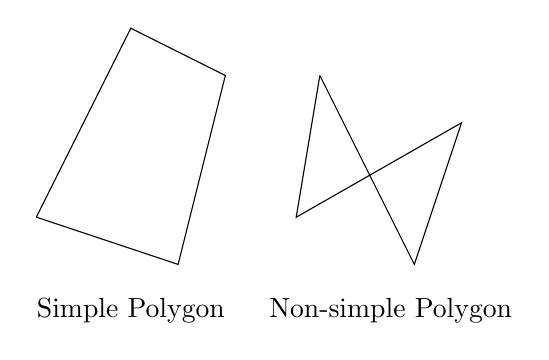
\begin{tikzpicture}[scale=0.6]
					\draw (0, 0) -- (3, -1) -- (4, 3) -- (2, 4) -- (0, 0);
					\draw (6, 3) -- (8, -1) -- (9, 2) -- (5.5, 0) -- (6, 3);
					\node at (2, -1.5) [below] {Simple Polygon};
					\node at (7.5, -1.5) [below] {Non-simple Polygon};
				\end{tikzpicture}
			\end{figure}

			Polygons are basic building blocks in most geometric applications. It can model arbitrarily complex shapes, and apply simple algorithms and algebraic representation/manipulation.
			
		\section{Triangulation}
			\begin{definition}[Triangulation]
				\textbf{Triangulation} is to partition polygon $P$ into non-overlapping triangles using diagonals only. It reduces complex shapes to collection of simpler shapes. Every simple $n$-gon admits a triangulation which has $n-2$ triangles.				
			\end{definition}

			\begin{figure}[h!]
				\centering
				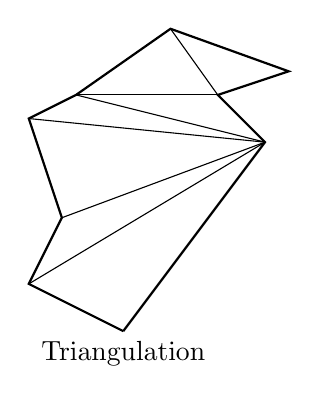
\begin{tikzpicture}[scale=0.6]
					\draw [thick] (0, 0) -- (3, 4) -- (2, 5) -- (3.5, 5.5) -- (1, 6.4) -- (-1, 5) -- (-2, 4.5) -- (-1.3, 2.4) -- (-2, 1) -- (0, 0);
					\draw (-2, 1) -- (3, 4);
					\draw (-1.3, 2.4) -- (3, 4);
					\draw (-2, 4.5) -- (3, 4);
					\draw (-1, 5) -- (3, 4);
					\draw (-1, 5) -- (2, 5);
					\draw (2, 5) -- (1, 6.4);
					\node at (0, 0) [below] {Triangulation};
				\end{tikzpicture}
			\end{figure}

			\begin{theorem}
				Every polygon has a triangulation				
			\end{theorem}

			\begin{lemma}
				Every polygon with more than three vertices has a diagonal.
			\end{lemma}

			\begin{proof}
				(by Meisters, 1975) Let $P$ be a polygon with more than three vertices. Every vertex of a $P$ is either \textit{convex} or \textit{concave}. W.L.O.G.(any polygon must has convex corner) Assume $p$ is a convex vertex. Denote the neighbors of $p$ as $q$ and $r$. If $\bar{qr}$ is a diagonal, done, and we call $\triangle{pqr}$ is an \textit{ear}. If $\triangle{pqr}$ is not an ear, it means at least one vertex is inside $\triangle{pqr}$, assume among those vertexes inside $\triangle{pqr}$, $s$ is a vertex closest to $p$, then $\bar{ps}$ is a diagonal.
			\end{proof}
			
		\section{Art Gallery Theorem}
			\begin{theorem}
				Every $n$-gon can be guarded with $\lfloor \frac{n}{3} \rfloor$ vertex guards
			\end{theorem}

			\begin{lemma}
				Triangulation graph can be 3-colored.
			\end{lemma}

			\begin{problem}
				The floor plan of an art gallery modeled as a simple polygon with $n$ vertices, there are guards which is stationed at fixed positions with 360 degree vision but cannot see through the walls. How many guards does the art gallery need for the security? (Fun fact: This problem was posted to Vasek Chvatal by Victor Klee in 1973).				
			\end{problem}

			\begin{proof}
				- $P$ plus triangulation is a planar graph\\
				- 3-coloring means there exist a 3-partition for vertices that no edge or diagonal has both endpoints within the same set of vertices.\\
				- Proof by Induction:\\
				\indent - Remove an ear (there will always exist ear) \\
				\indent - Inductively 3-color the rest\\
				\indent - Put ear back, coloring new vertex with the label not used by the boundary diagonal.
			\end{proof}

		\section{Triangulation Algorithms}

		\section{Shortest Path}


